%----------------------------------------------------------------------------------------
%	PACKAGES AND OTHER DOCUMENT CONFIGURATIONS
%----------------------------------------------------------------------------------------

\documentclass[12pt]{article}
\usepackage{polski}
\usepackage[polish]{babel}
\usepackage[utf8]{inputenc}
\usepackage{datetime}
\usepackage{graphicx}
\usepackage{tikz}
\usepackage{amsmath}
\usepackage{multirow}
\usepackage{tabularx}
\usepackage{geometry}
\usepackage{subcaption}
\usepackage{epstopdf}
% Real R
\usepackage{amsfonts}

\bibliographystyle{unsrt}

\geometry{
 	a4paper, 
 	left    = 20mm,
 	right	  = 20mm,
 	top     = 20mm,
 	bottom  = 20mm,
}
 
%----------------------------------------------------------------------------------------
 
%----------------------------------------------------------------------------------------
% DATES
%----------------------------------------------------------------------------------------

\renewcommand{\dateseparator}{.}
\newdate{exercise_date}{08}{03}{2016}


% dodatkowe typy kolumn tabel

% flush left fixed width:
\newcolumntype{L}[1]{>{\raggedright\arraybackslash}p{#1}}

% center fixed width:
\newcolumntype{C}[1]{>{\centering\arraybackslash}p{#1}}

% flush right fixed width:
\newcolumntype{R}[1]{>{\raggedleft\arraybackslash}p{#1}}

%----------------------------------------------------------------------------------------

%----------------------------------------------------------------------------------------
% TIKZ PACKAGES
%----------------------------------------------------------------------------------------

\usetikzlibrary{arrows}

%----------------------------------------------------------------------------------------

\begin{document}
 
\begin{titlepage}

\newcommand{\HRule}{\rule{\linewidth}{0.5mm}}
% Defines a new command for the horizontal lines, change thickness here

\center
% Center everything on the page
 
%----------------------------------------------------------------------------------------
%	LOGO SECTION
%----------------------------------------------------------------------------------------


\includegraphics[width=6cm]{../res/img/logo.png}\\[1cm]
% Include a department/university logo - this will require the graphicx package
 
%----------------------------------------------------------------------------------------
 
%----------------------------------------------------------------------------------------
%	HEADING SECTIONS
%----------------------------------------------------------------------------------------

\textsc{\LARGE Akademia Górniczo-Hutnicza \\[0.2cm]
im. Stanisława Staszica w Krakowie}\\[1.5cm]
% Name of your university/college

\textsc{\Large Optymalizacja w systemach sterowania}\\[0.5cm]
% Major heading such as course name

%----------------------------------------------------------------------------------------
%	TITLE SECTION
%----------------------------------------------------------------------------------------

\HRule \\[0.5cm]
{ \huge \bfseries Lewitacja magnetyczna - sterowanie docelowe}\\[0.3cm]
% Title of your document
\HRule \\[1.5cm]

\flushright
\Large \emph{Prowadzący:}\\
dr inż. Piotr \textsc{Bania}\\[1cm]
\Large \emph{Autorzy:}\\
Anna \textsc{Musiał}\\[0.1cm]  % Your name
Grzegorz \textsc{Król}\\[0.1cm]        % Your name
Filip \textsc{Kubicz}\\[0.1cm]
Kazimierz \textsc{Chudzik}\\[3cm]
% Authors


%----------------------------------------------------------------------------------------
%	DATE SECTION
%----------------------------------------------------------------------------------------
% Data wykonania ćwiczenia: \\
% {\large \displaydate{exercise_date}}\\[1cm]


\vfill % Fill the rest of the page with whitespace

\end{titlepage}
Plan działania: \\

\begin{enumerate}
\item Obsługa enkoderów.
\item Obsługa tachoprądnicy.
\item Sterowanie silników.
\item Obliczenie analityczne parametrów $I_h, I_v$.
\item Identyfikacja parametrów oraz zależności: \\
- tarcie (wahadła) $k_m, k_v$ \\
- charakterystyki $F_m, F_t, \omega_m, \omega_t$ 
\item Synteza regulatorów.
\item Badania symulacyjne.
\item Weryfikacja modelu – zamiana modelu na sprzęt.
\item Realizacja zadania stabilizacji statycznej lub dynamicznej.
\item Ocena jakości regulacji i dyskusja nad użytymi regulatorami.
\end{enumerate}

\section{Model matematyczny stanowiska MagLev}

Lewitacja magnetyczna to zjawisko występujące, kiedy ferromagnetyczny obiekt znajdzie się w polu magnetycznym skierowanym pionowo w górę, na tyle silnym, że wytworzona siła zrównoważy działającą na przedmiot grawitację. Zjawisko to stosuje się obecnie w łożyskach magnetycznych w pociągach, rozwijanych głównie w Japonii (MLX01) i w Niemczech (TR-08).

W laboratorium Katedry Automatyki EAIiIB AGH znajduje się stanowisko przeznaczone do badania magnetycznej lewitacji. Obiektem unoszącym się jest metalowa sfera. Pole magnetyczne jest wytwarzane przez cewkę umieszczoną ponad sferą. Dzięki pracom \cite{Bania1999}, \cite{Bania2000} i \cite{Pilat} wiemy w jaki sposób modelować zachowanie układu, a także identyfikować jego parametry fizyczne.

\begin{figure}[!htb]
\centering
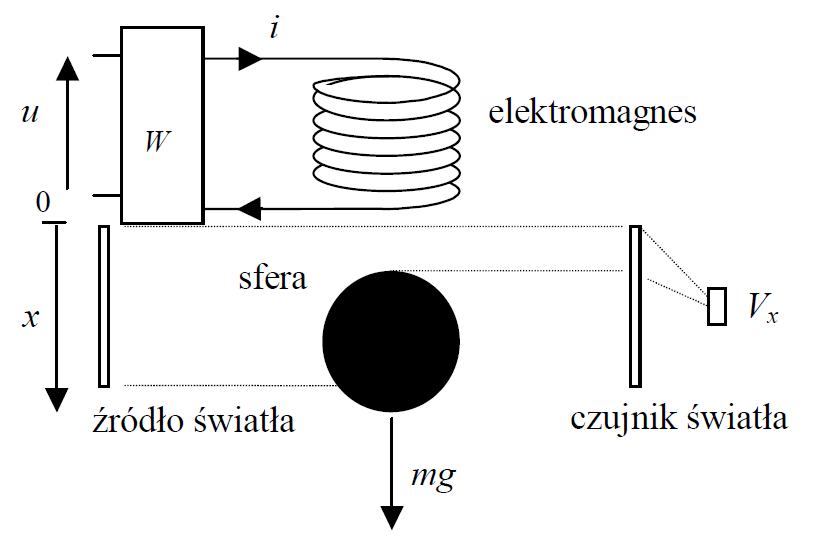
\includegraphics[scale=0.45]{img/model-rownania.PNG}
\caption{Schemat stanowiska służący do wyznaczania równań, źródło \cite{Bania200.}}
\label{rys:model-rownania}
\end{figure}

\begin{equation}\label{modelMagLev}
  \begin{cases}
    \dot x_1 & = x_2 \\
    \dot x_2 & = \dfrac{1}{2m} \dfrac{dL(x_1)}{dx_1} x_3^2(t) + 10^{-3} g  \\
    \dot x_3 & = -\frac{1}{T} x_3(t) + \frac{k}{T} (u(t) + u_c) \\
  \end{cases}  
\end{equation}

Gdzie:
\\$x_{1}$ - położenie sfery $[m]$
\\$x_{2}$ - prędkość sfery $[m/s]$
\\$x_{3}$ - prąd w cewce $[A]$ \newline

\subsection{Analiza modelu}

Zmienne stanu i sterowanie spełniają warunki:
\begin{equation}
\begin{cases}
x_1(t) \in [0, x_{max}] \\
x_2(t) \in R \\
x_3(t) \in [ku_c, k(u_c+u_{max})] \\
u(t) \in [0, u_{max}]
\end{cases}
\end{equation}




\section{Sterowanie optymalne}

Jeżeli układ nieliniowy ma postać
\begin{equation}
\dot{x} = f(x) + g(x) \cdot u, \qquad x \in \mathbb{R}^n, u \in \mathbb{R}^n, t \in [0,T], f \in C^1
\end{equation}
z warunkiem początkowym
\begin{equation}
x(0) = x_0
\end{equation}
To przyjmując wskaźnik jakości w formie funkcjonału
\begin{equation} \label{wskaznik}
J(u, T) = q(T, x(T)) = T + \frac{1}{2} \rho |x(T) - x_{ref}|^2
\end{equation}
\textbf{sterowanie optymalne}, tj. takie, które najszybciej doprowadza układ do zadanego położenia ma postać sterowania bang-bang
\begin{equation}
u(t) = 
\begin{cases}
    u_{max}, g^T \psi > 0 \\
    u_{min}, g^T \psi < 0
\end{cases}
\end{equation}
Przyjęto że czasy przełączeń sterowania oznaczono przez $\tau_1, \tau_2, ..., \tau_n, T$.

\noindent
$\psi(t)$ to funkcja oznaczająca równanie sprzężone układu, takie że
\begin{equation}
\dot{\psi} = - \nabla_x H
\end{equation}
gdzie $H$ jest macierzą Hamiltona układu.

Sprawdzenie, czy sterowanie jest optymalne może być przeprowadzone przez wyrysowanie \textbf{funkcji przełączającej} i jej porównanie ze sterowaniem. Funkcja przełączająca ma postać
\begin{equation}
\Phi(t) = g^T(x(t)) \cdot \psi(t)
\end{equation}

\subsection{Analiza układu MagLev}

Hamiltonian układu \ref{maglev_rown} ma postać
\begin{equation}
H = \psi_1 x_2 + \psi_2 (bx_3^2 e^{ax_1}+g) + \psi_3 (cx_3 + u)
\end{equation}

Równania sprzężone układu magnetycznej lewitacji  \cite{Turnau}:
\begin{equation}
\begin{cases}
	\dot{\psi}_1 = - ab \cdot e^{ax_1} \cdot x_3^2 \psi_2 \\
	\dot{\psi}_2 = - \psi_1 \\
	\dot{\psi}_3 = -2b \cdot e^{ax_1} \cdot x_3 \psi_2 - c \psi_3
\end{cases}
\end{equation}

W celu przyspieszenia numerycznej optymalizacji sterowania z użyciem funkcji fmincon() z pakietu Optimization \textsc{MATLAB}a, należy obliczyć gradient wskaźnika jakości względem czasów przełączeń. Gradient wskaźnika jakości po czasach przełączeń $\tau_i$ dla układu MagLev jest dany wzorem
\begin{equation}
\nabla_{\tau_i} J = \Phi(t) (u^+ - u^-)
\end{equation}
Natomiast gradient wskaźnika jakości po czasie końcowym ma postać
\begin{equation} \label{gradient}
\nabla_T J = 1 - H(\psi(T), x(T), u(T^-))
\end{equation}

%\begin{figure}[!htb]
%  \begin{center}
%    \includegraphics[width=14.5cm,trim=1.6cm 6.9cm 1.7cm 8.5cm,clip]
%    {img/exp_omega.pdf}
%  \end{center}
%  \caption{Eksperyment wyznaczenia charakterystyk prędkości śmigieł od napięcia na silnikach przy zablokowanych osiach}
%  \label{plot:exp1}
%\end{figure}






\section{Optymalizacja w środowisku \textsc{MATLAB}}

Model matematyczny i znajomość struktury optymalnego sterowania bang-bang wykorzystano do numerycznej optymalizacji wskaźnika jakości określającego jak najszybsze dotarcie do zadanego położenia równowagi.

Rozwiązywanie równań w środowisku \textsc{MATLAB}...

%\begin{figure}[!htb]
%\centering
%\includegraphics[scale=0.85]{img/symulacja_simulink.png}
%\caption{Model numeryczny w środowisku \textsc{Simulink}}
%\label{rys:sim_simulink}
%\end{figure}

\subsection{Wykorzystanie ustawień fmincon()}




\section{Wnioski}

Sterowanie docelowe metodą QTO-RHC pozwala na predykcję funkcji sterującej dla obiektów nieliniowych. 
Często znalezienie sterowania optymalnego jest trudnym zadaniem, które wymaga dużych nakładów 
obliczeniowych i czasowych. Naszym zadaniem optymalizacji była stabilizacja położenia i prędkości metalowej
kulki lewitującej w polu magnetycznym. W trakcie laboratoriów wykorzystywano algorytm Rungego-Kutty, za 
pomocą którego rozwiązywano równania różniczkowe "w przód" oraz "wstecz". Została napisana funkcja do
obliczania wskaźnika jakości wraz z gradientami, która następnie została poddana minimalizacji przy pomocy
funckji fmincon programu Matlab. Jako jedną z opcji funkcji fmincon ustawiono wykorzystanie obliczanego 
wewnątrz funkcji celu gradientu wskaźnika jakości. Przyspieszyło to znalezienie sterowania odpowiadającego
założeniom projektowym. Rozwiązanie problemu optymalizacji było możliwe dzięki wcześniejszej znajomości
modelu matematycznego rozważanego obiektu wraz z równaniami stanu i sprzężonymi. 



\bibliography{chapters/Bibliografia}

\end{document}